\documentclass[landscape]{article}
\usepackage[pdftex]{graphicx}
\pagestyle{empty}
\oddsidemargin  -0.5 in
\evensidemargin -0.5 in
\headheight     0 in
\topmargin      -1 in
\textheight     7.7 in
\textwidth      10 in
\newenvironment{slide}{\mbox{ }\vfill}{\vfill \mbox{ } \pagebreak}
\newenvironment{lastslide}{\mbox{ }\vfill}{\vfill \mbox{ }}
\begin{document}
\Huge
\renewcommand{\labelitemi}{-}
\renewcommand{\labelenumii}{\alph{enumii}.}
\setlength{\parindent}{0 cm}

\begin{slide}
\begin{center}

\includegraphics[width=0.9\linewidth]{title} \\
Jim Pivarski
\end{center}
\end{slide}

\begin{slide}
  Table of Contents

  \vfill
  \begin{center}
    \begin{minipage}{22 cm}
      \begin{enumerate}\setlength{\itemsep}{0.5 cm}
        
        \item Review of the detector

	\item What is Suez/the Event Display?

        \item Running Suez with a tcl file (demonstration)

        \item A look at CLEO {\it within} the Event Display (demo)

        \item Some things you can do to the Event Display (demo)

        \item Doing something with your processor: histograms (demo)

        \item Filtering with your processor (demo)

        \item Tools (and facts) available for physics

        \item ``Homework''

      \end{enumerate}
    \end{minipage}
  \end{center}

  \vfill
\end{slide}

\begin{slide}
\begin{center}
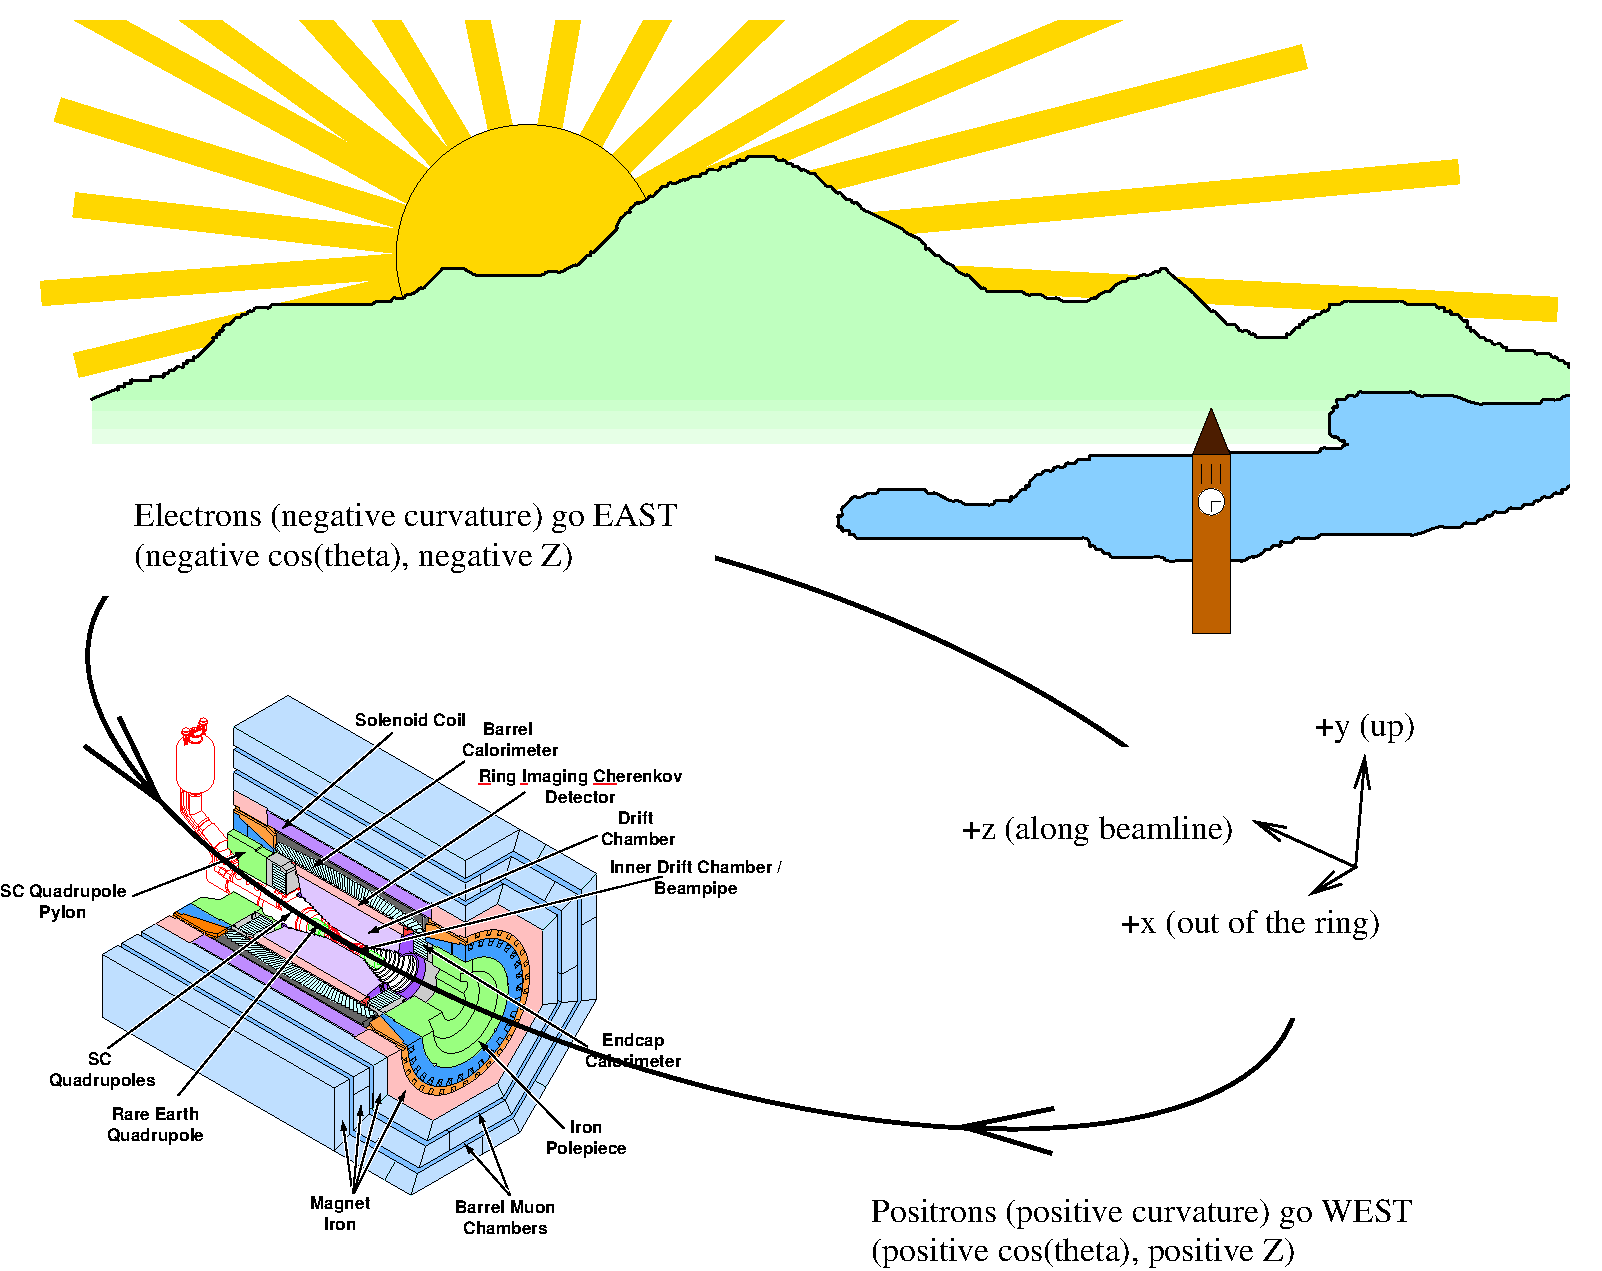
\includegraphics[width=0.85\linewidth]{cleo_detector}
\end{center}
\end{slide}

\begin{slide}
Your plaything:

\begin{center}
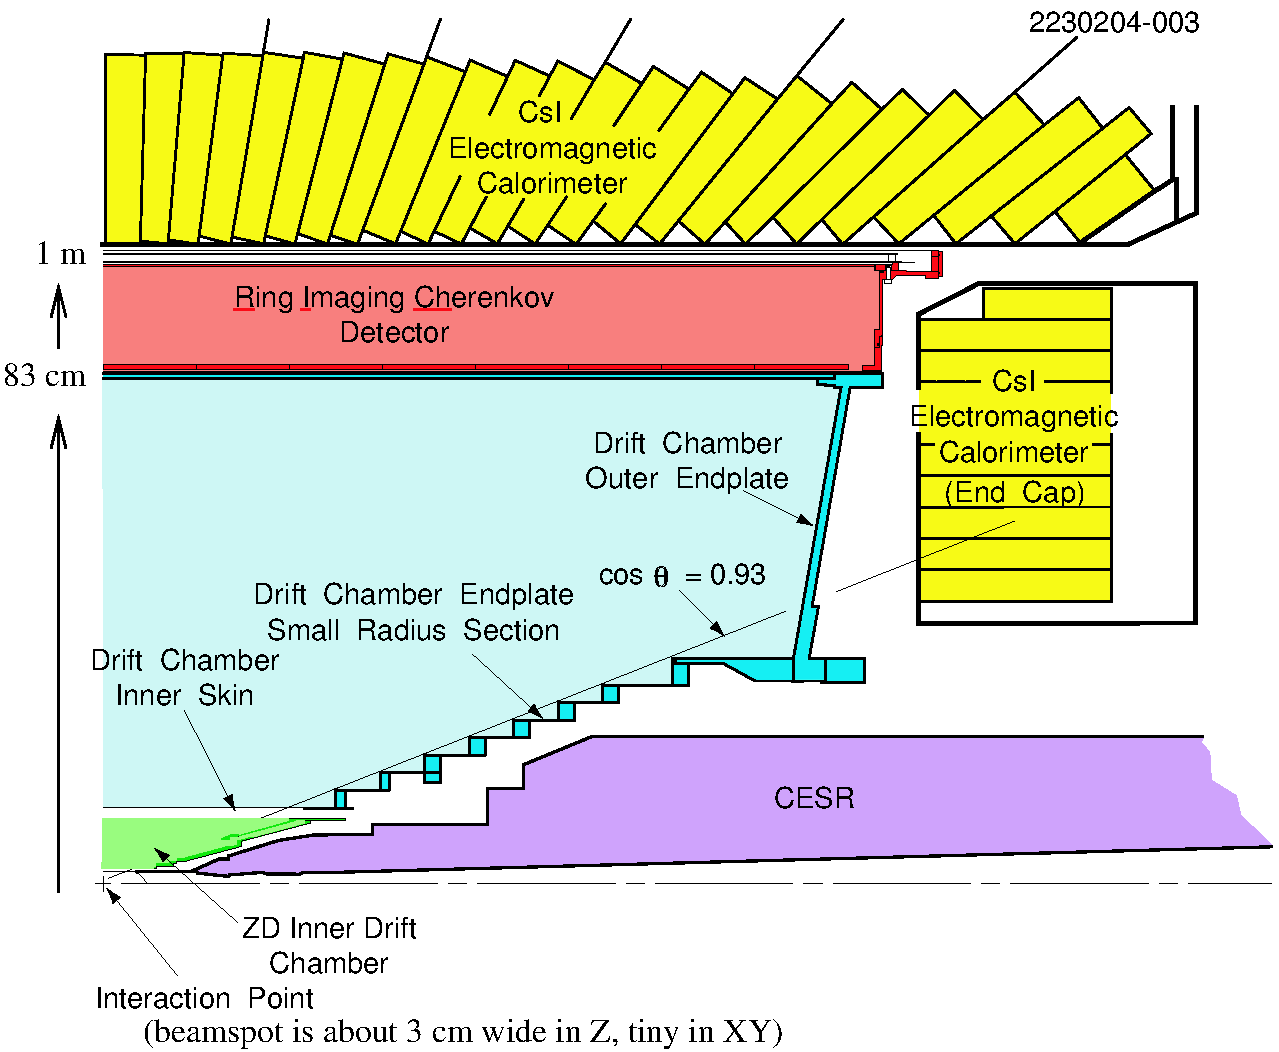
\includegraphics[width=0.75\linewidth]{quarter_view2}
\end{center}
\end{slide}

\begin{slide}
What is Suez?

\vspace{1 cm}
\begin{center}
  \begin{minipage}{0.9\linewidth}
    A commandline-driven program that unifies all CLEO code.  All CLEO
    data is accessible inside Suez, and all algorithms can be accessed
    by dynamically loading modules (``producers'').

    \vspace{1 cm}
    We will always run Suez as a batch process: we will put all of our
    commands into a {\tt .tcl} file and run it by
    \begin{center} \tt suez -f whatever.tcl \end{center}

    \vspace{1 cm}
    You will write a ``processor'' ({\tt e.g.\ MyFirstProc}) which is
    C++ code that is executed on every event.  In your processor, you
    will get data with an {\tt extract} command, which executes code
    in the producers that you dynamically loaded (or crash, if you
    forgot to do that).  The producers might just read the data off
    the disk and give it to you, or they might do some processing
    first.
  \end{minipage}
\end{center}
\end{slide}

\begin{slide}
  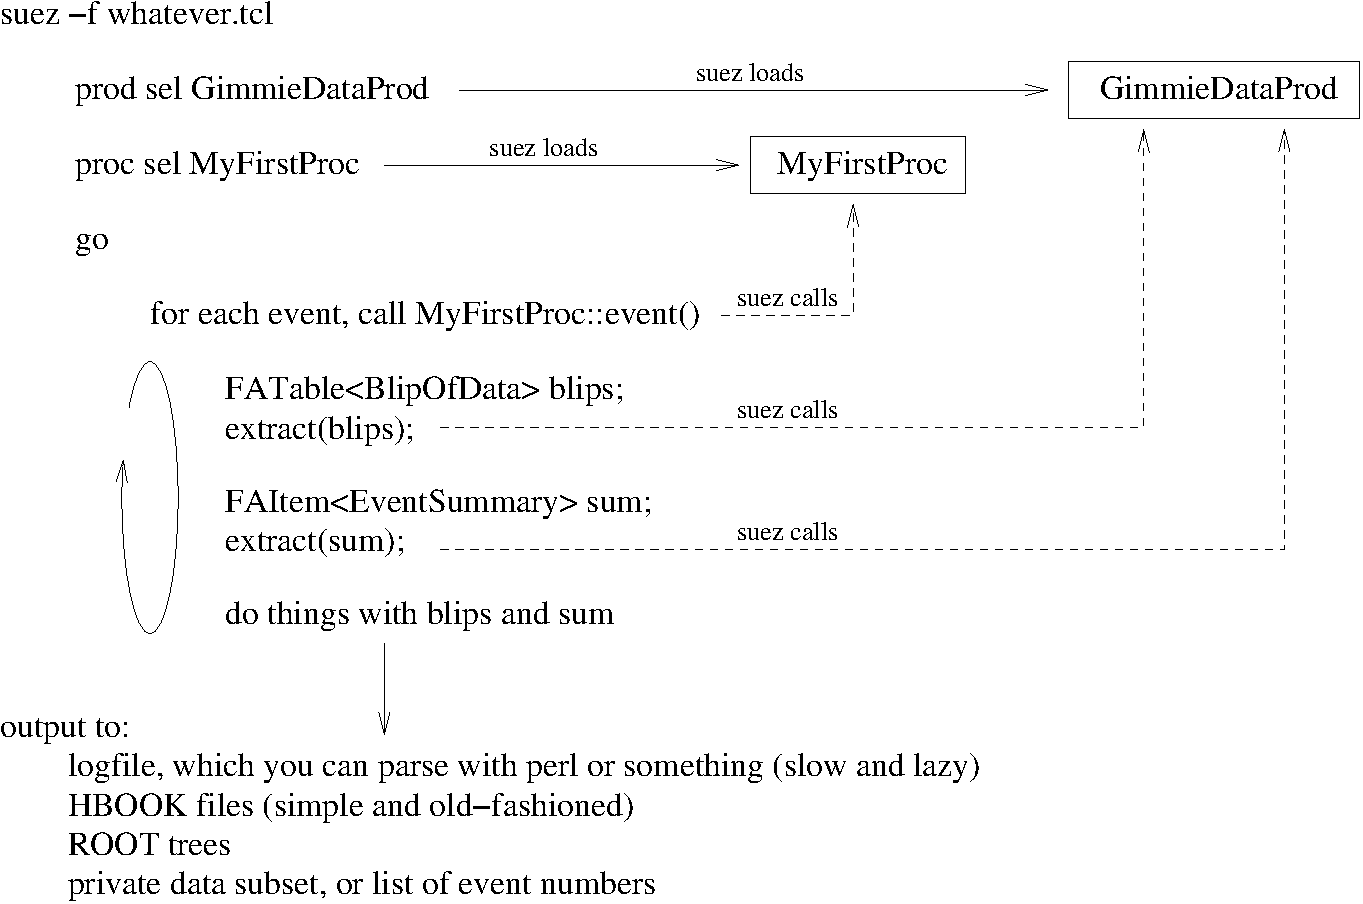
\includegraphics[width=\linewidth]{suezwork}
\end{slide}

\begin{slide}
What is the Event Display?

\vspace{0.5 cm}
\begin{center}
  \begin{minipage}{0.9\linewidth}
    An event-by-event viewer written as a collection of Suez
    processors (accessible by a single command).

    \vspace{0.8 cm}
    Because everything is dynamically-loadable, you can run your
    processor AND look at the same events in the Event Display.

    \vspace{0.8 cm}
    It will be most useful to you as a diagnostic: when you can't
    figure out what's wrong with your plots but you can define
    selection criteria (``cuts'') to pick out the problem events, to
    see what they look like.  It is constantly running during
    data-taking.
  \end{minipage}
\end{center}

\vspace{0.8 cm}
What is HistogramViewerProc?

\vspace{0.5 cm}
\begin{center}
  \begin{minipage}{0.9\linewidth}
    It's a processor that we'll use to look at histograms while still
    running over data.  Usually, you'll output all of your data in
    some interactive format (HBOOK, ROOT\ldots) and make your
    histograms outside of Suez.
  \end{minipage}
\end{center}
\end{slide}

\begin{slide}
``Useful facts'' (first page of the exam)

\vfill
Jackson p.\ 582 (the useful page):

\vspace{-1 cm}
\begin{eqnarray*}
p_T &=& 3.00 \times 10^{-4} \, \mbox{(MeV/$c$/gauss/cm) } B \times R \\
p_T &=& 0.3 \, \mbox{(GeV/$c$/m)} \times R
\end{eqnarray*}

where $R = 1/2/$curvature and $B_{\mbox{\normalsize CLEO}} \approx
9.94 \mbox{ kgauss}$.

\vfill
Isotropic (radially-symmetric) decays are uniform in $\cos\theta$.

\vfill
If no particles are lost or double-counted,
\begin{itemize}
  \item Total energy is 2 $\times$ beam energy
  \item Total momentum is almost (0, 0, 0) (there's a {\it small} crossing angle)
  \item Total charge is zero
  \item \begin{tabular}{p{0.5\linewidth} p{0.23\linewidth} p{0.23\linewidth}}
    \mbox{\hspace{-0.4 cm}} \begin{minipage}{\linewidth} Total angular momentum is $J=1$: \end{minipage} &
    \begin{minipage}{\linewidth} 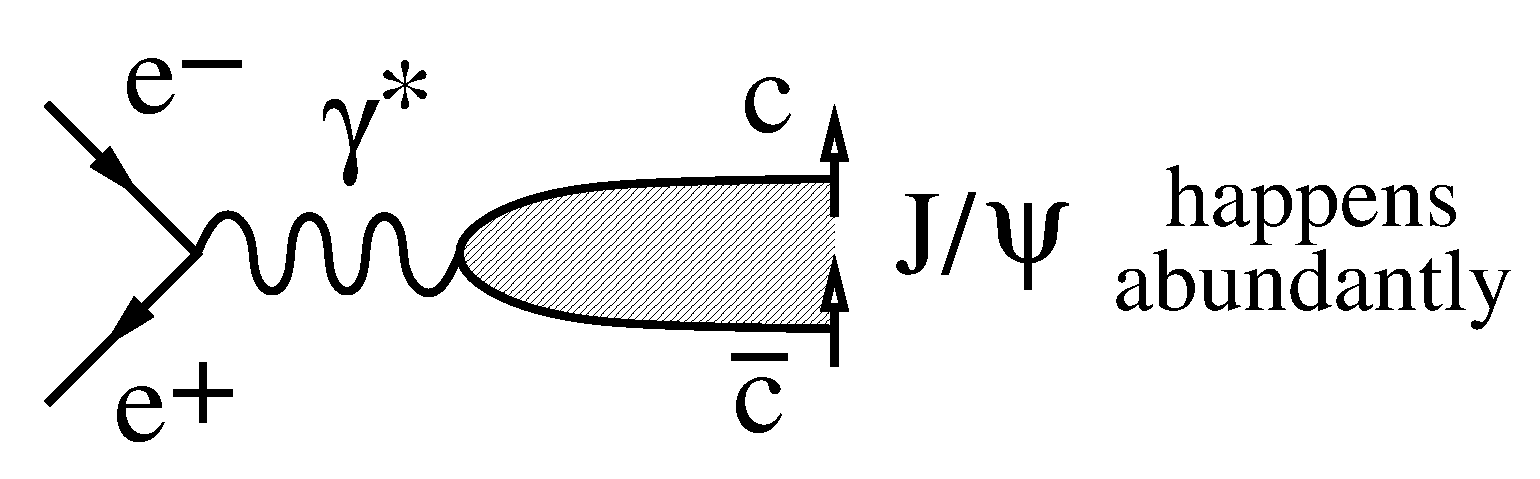
\includegraphics[width=\linewidth]{diagram_jpsi} \end{minipage} &
    \begin{minipage}{\linewidth} 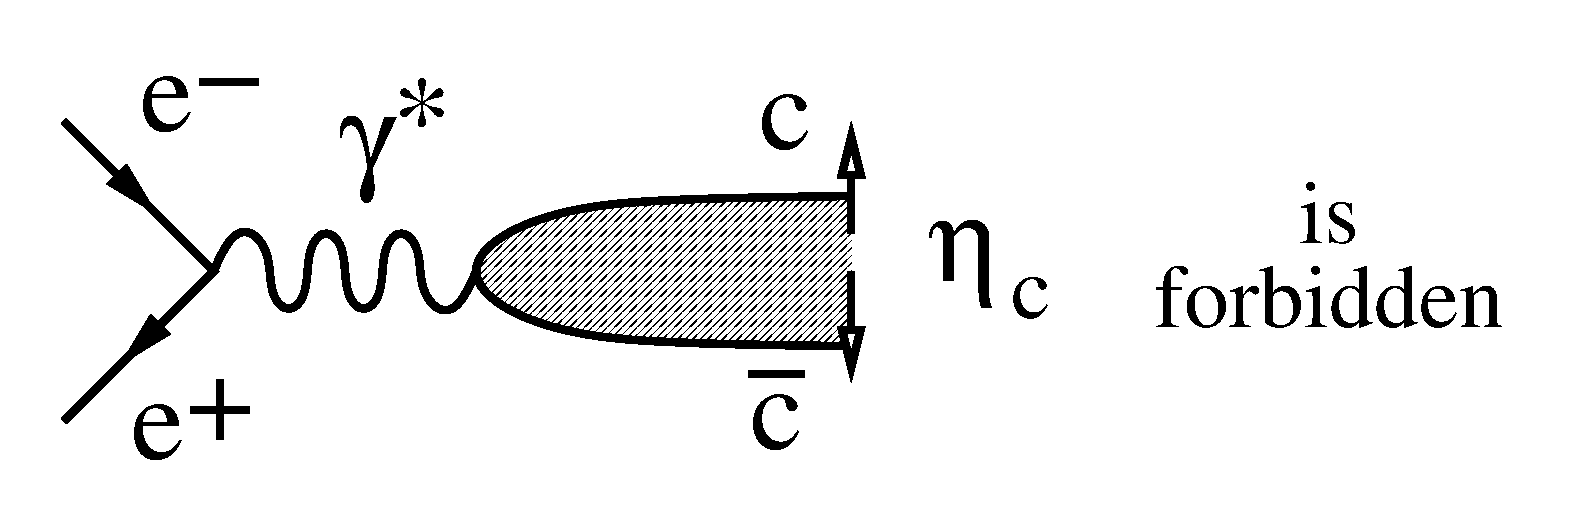
\includegraphics[width=\linewidth]{diagram_etac} \end{minipage}
  \end{tabular}
\end{itemize}

\end{slide}

%% \begin{slide}
%% What that would look like, if we waited long enough (and if no bhabhas
%% or cosmic rays leaked through)

%% \vfill
%% 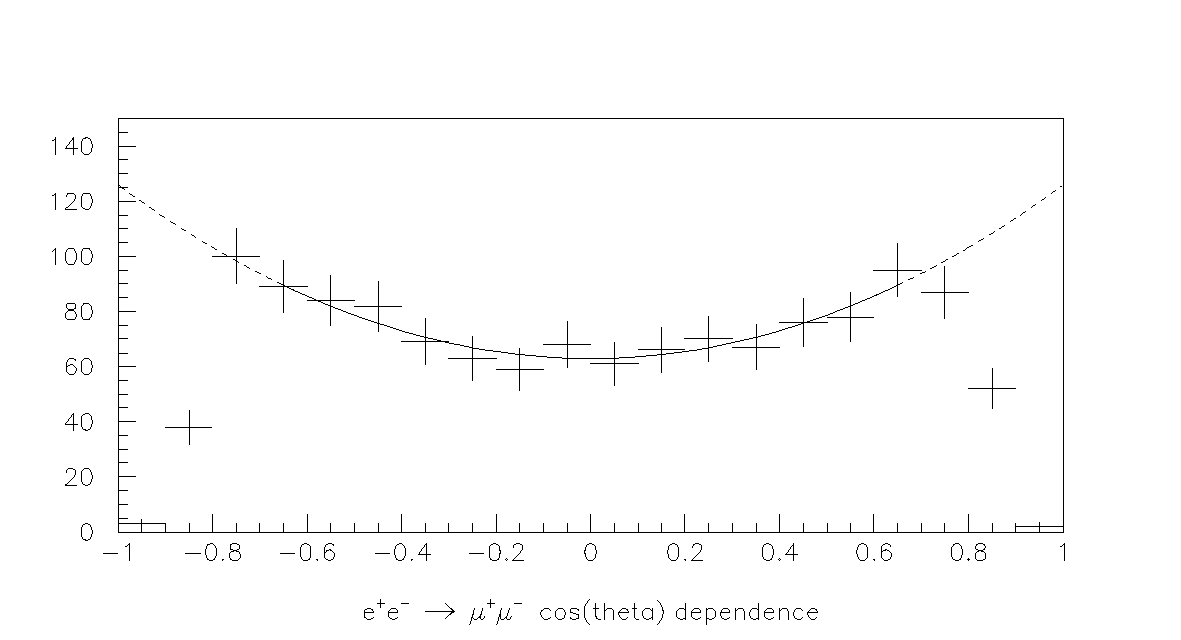
\includegraphics[width=\linewidth]{mupair_costh}
%% \end{slide}

\begin{slide}
\huge

Momentum from {\tt trackItr->pionFit()->}
\begin{itemize}
  \item {\tt momentum()}: a {\tt HepVector3D} (``$+$'' and ``$*$'' do linear algebra)
  \item {\tt momentum().x()}, {\tt momentum().y()}, {\tt momentum().z()}
  \item {\tt momentum().mag()}: $|\vec{p}|$
  \item {\tt momentum().perp()}: $p_T$ (magnitude of projection onto XY)
\end{itemize}

\vspace{-2 cm}
\begin{flushright}
  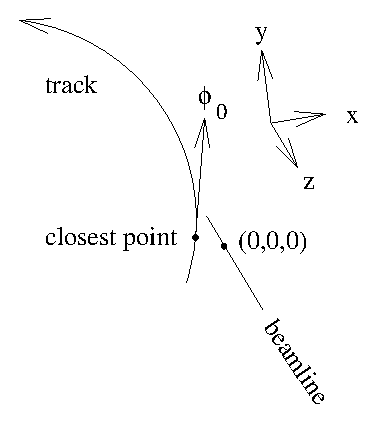
\includegraphics[width=6 cm]{track_parameters}
\end{flushright}

\vspace{-5 cm}
Track parameters (from {\tt trackItr->pionHelix()->})
\begin{itemize}
  \item {\tt curvature()} in m$^{-1}$: remember the factor of 2!
  \item {\tt d0()}: distance of closest approach to (0,0,0) in XY plane (signed)
  \item {\tt z0()}: distance of closest approach to (0,0,0) in Z (signed, of course)
  \item {\tt phi0()}: angle in XY closest to (0,0,0) (ranges from 0 to $2\pi$)
  \item {\tt cotTheta()}: $\displaystyle \cot\theta = \frac{\cos\theta}{1 -
  \cos^2\theta}$ and $\displaystyle \cos\theta = \frac{\cot\theta}{1 +
  \cot^2\theta}$
\end{itemize}

\vfill
\begin{minipage}{\linewidth}
\large {\tt http://www.lns.cornell.edu/restricted/webtools/doxygen/Offline/html/classTDTrack.html \\
http://www.lns.cornell.edu/restricted/webtools/doxygen/Offline/html/classNavTrack.html \\
http://www.lns.cornell.edu/restricted/webtools/cleo3/source/other\_sources/CLHEP/CLHEP/Vector/ThreeVector.h} \\
(don't worry about difference between {\tt Hep3Vector}, {\tt HepVector3D}, {\tt HepPoint3D}\ldots)
\end{minipage}
\end{slide}

\begin{slide}
\huge

Stuff from {\tt showerItr->attributes().} (note the dot, rather than arrow)
\begin{itemize}
  \item {\tt energy()} in GeV
  \item {\tt phi()} (0 to $2\pi$) and {\tt theta()}: assume shower came from the origin
  \item {\tt momentum()}: energy in direction $\phi$, $\theta$ ({\tt Hep3Vector})
  \item {\tt hot()}: this crystal is always on, and therefore not to
    be trusted
\end{itemize}

\vfill
Stuff from {\tt showerItr->}
\begin{itemize}
  \item {\tt noSimpleMatch()}: (boolean) no track came near this shower
  \item {\tt simpleMatch()}: nearest {\tt FAItem<NavTrack>} to this shower
  \item {\tt angSimpleMatch()}: angle between shower and track, if
    there is one
\end{itemize}

\vfill
Be careful!  Accessing {\tt simpleMatch()} when {\tt noSimpleMatch()}
is true will cause a segmentation fault.  A {\tt FAItem<NavTrack>} can
be used like a {\tt trackItr}:
\begin{center}
  {\tt showerItr->simpleMatch()->pionHelix()->d0()}, etc.
\end{center}
Also, you'd need {\tt \#include "Navigation/NavTkShMatch.h"} in your
{\tt .cc} and \\ {\tt TrackShowerMatching} in your {\tt Makefile}'s
{\tt CLEO3\_LIBS} to use track-shower matching.

\vfill
\begin{minipage}{\linewidth}
\large {\tt http://www.lns.cornell.edu/restricted/webtools/doxygen/Offline/html/classNavShower.html \\
http://www.lns.cornell.edu/restricted/webtools/doxygen/Offline/html/classCcShowerAttributes.html}
\end{minipage}
\end{slide}

\begin{slide}
\huge {\tt
\#include "CleoDB/DBEventHeader.h" \\
\#include "BeamEnergy/BeamEnergy.h" \\
\#include "BeamSpot/BeamSpot.h" \\
\#include "MagField/MagneticField.h"

\vspace{0.45 cm}
FAItem<DBEventHeader> eventHeader; \\
extract(iFrame.record(Stream::kEvent), eventHeader); \\
{\rm use} evenHeader->run() {\rm and} evenHeader->number() {\rm for
run and event numbers.}

\vspace{0.45 cm}
FAItem<BeamSpot> beamSpot; \\
extract(iFrame.record(Stream::kBeginRun), beamSpot); \\
{\rm use} beamSpot->center() {\rm (a HepPoint3D)}

\vspace{0.45 cm}
FAItem<MagneticField> magneticField; \\
extract(iFrame.record(Stream::kStartRun), magneticField); \\
{\rm use} magneticField->BField()

\vspace{0.45 cm}
FAItem<BeamEnergy> beamEnergy; \\
extract(iFrame.record(Stream::kStartRun), beamEnergy); \\
{\rm use} beamEnergy->value()}

\vspace{0.45 cm}
These require {\tt CleoDB}, {\tt BeamEnergy}, {\tt BeamSpot}, and {\tt
MagField} in your {\tt Makefile}.
\end{slide}

\begin{slide}
Very important webpages/places to look for things:

\vfill
Finding out what member functions are available: \\
{\tt \LARGE http://www.lns.cornell.edu/restricted/webtools/doxygen/Offline/html/hierarchy.html}

\vfill
Looking at the code: \\
{\tt \LARGE http://www.lns.cornell.edu/restricted/webtools/cleo3/} \\
{\tt \LARGE ls \$C3\_CVSSRC/} (DON'T TAB-TAB!) \\
{\tt \LARGE ls \$C3\_OTHER/}

\vfill
Finding out what producer you need to add to your {\tt .tcl}: \\
{\tt \LARGE http://www.lns.cornell.edu/$\sim$cleo3/current/data/proxiesOfProducers.txt}

\vfill
Finding out what cuts have already been applied to your data: \\
{\tt \LARGE http://www.lns.cornell.edu/restricted/CLEO/CLEO3/soft/hints/
\begin{flushright} CLEOIIIEventClassificationDescription.html \end{flushright}}

\end{slide}

\begin{slide}
\begin{center}
  \begin{tabular}{p{0.45\linewidth} p{0.5\linewidth}}
    \begin{center} Energy loss in the drift chamber \end{center} &
    \begin{center} Ring-Imaging \v{C}erenkov Detector \end{center} \\
    \begin{minipage}{\linewidth} \vspace{-0.5 cm} \begin{center} 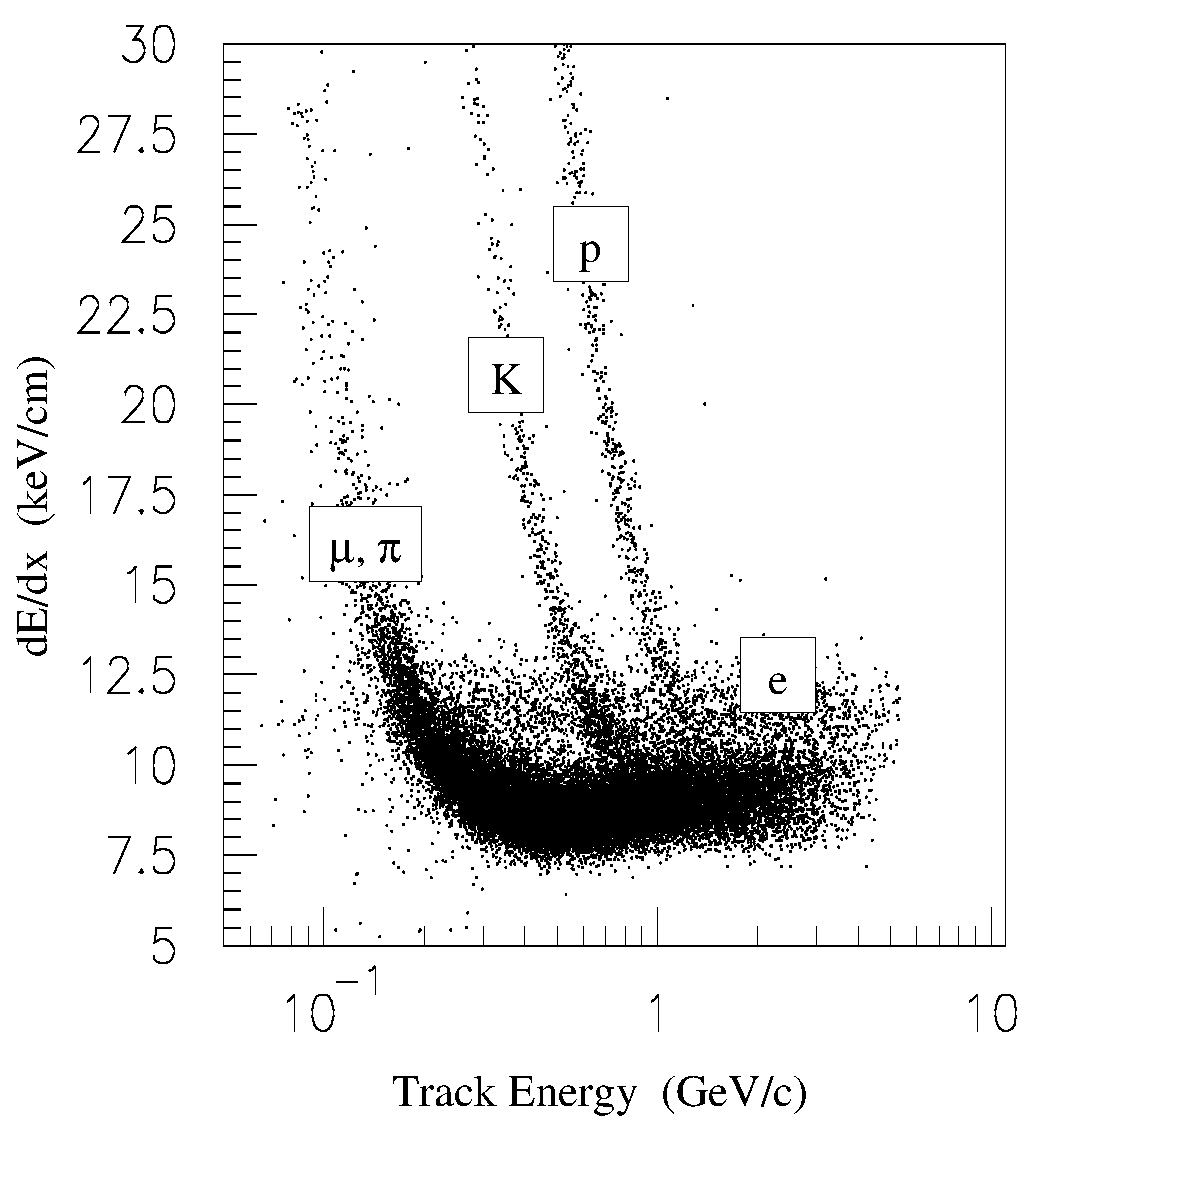
\includegraphics[height=12.5 cm]{dedx} \end{center} \end{minipage} &
    \begin{minipage}{\linewidth} \vspace{-1.3 cm} \begin{center} 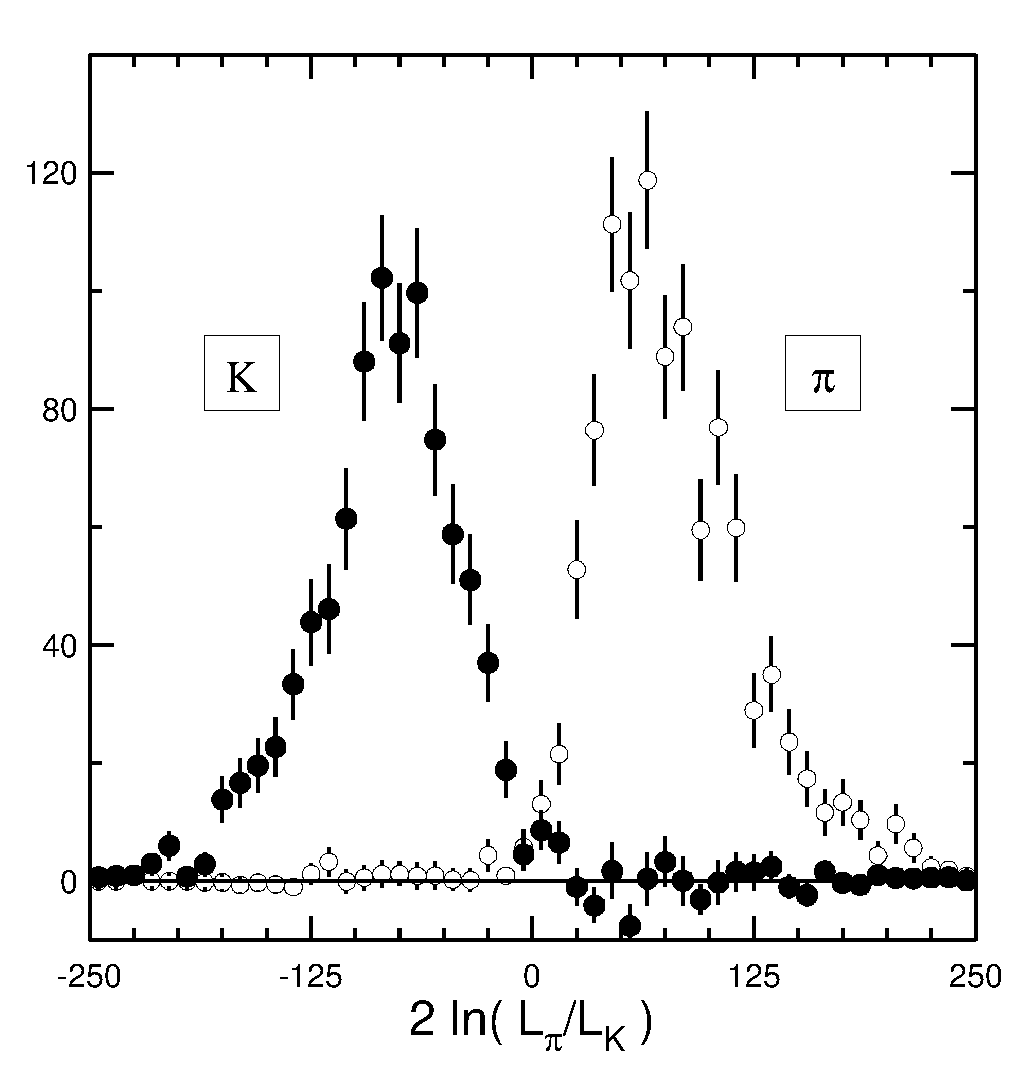
\includegraphics[height=11.5 cm]{rich_kpisep2} \end{center} \end{minipage} \\
    \begin{center} \tt trackItr->dedxInfo() \end{center} & \begin{center} \tt trackItr->richInfo() \end{center} \\
  \end{tabular}
\end{center}
\end{slide}

\begin{slide}
{\bf Homework} (that you do here, not at home)

\begin{enumerate}\setlength{\itemsep}{1 cm}

  \item Run the Event Display on hits and everything, and
    \begin{enumerate}
      \item under View, select Create Info View and see what happens when you
	select hits and tracks;

      \item select all SeedTracks in the Hierarchy View and make them
	invisible (under Action menu);

      \item with Set 2D Representation, turn all CCShowerAttributes
	(showers) into momentum vectors at the origin and KinePionFits
	(fitted tracks) into momentum vectors originating at their
	``position,'' then step through a few events.  When a shower
	clearly belongs to a pair of tracks that made them, why do the
	arrows sometimes not line up?

      \item Again with Set 2D Representation, turn the
	CalibratedDRHits into lines from endPoint1 to endPoint2 and
	look at them in the front and side views.  Which ones are the
	stereo hits?  From Select$\to$Select by Data, select
	CalibratedDRHits with layer number $\ge$ 17 (stereo).
    \end{enumerate}
\end{enumerate}
\end{slide}

\begin{slide}
{\bf Homework continued} (slightly more difficult, but you should do
at least one)

\vfill
\begin{enumerate}\setlength{\itemsep}{1 cm}
  \addtocounter{enumi}{1}
  \item Show me an event display of $e^+e^- \to e^+e^-\gamma$, a
    really dramatic one, with $E_\gamma \sim E_{e^\pm}$.  These are
    rare, so you'll have to make a filtering processor to find them.

  \item Plot $\cos\theta$ of $e^+e^- \to \gamma\gamma$ (and compare
    Peskin and Schroeder p.\ 169--- I have a copy).

  \item The two incident beams don't collide exactly head on, but at a
    slight angle.  Measure this momentum offset (hint: it will be
    $\sim$10 MeV).  What is the direction of this offset?

  \item Plot $\displaystyle \sum p_z$ for events in which one incident
    beam hits a gas atom (``beam-gas'').  What cuts would identify an
    event that comes from the beam but not the beam collision point?

\end{enumerate}

\end{slide}

\begin{slide}
\huge {\bf Advanced homework:} hunt for strange particles!
($\Lambda \to p \pi^-$ or $K^0_S \to \pi^+\pi^-$)

\begin{center}
  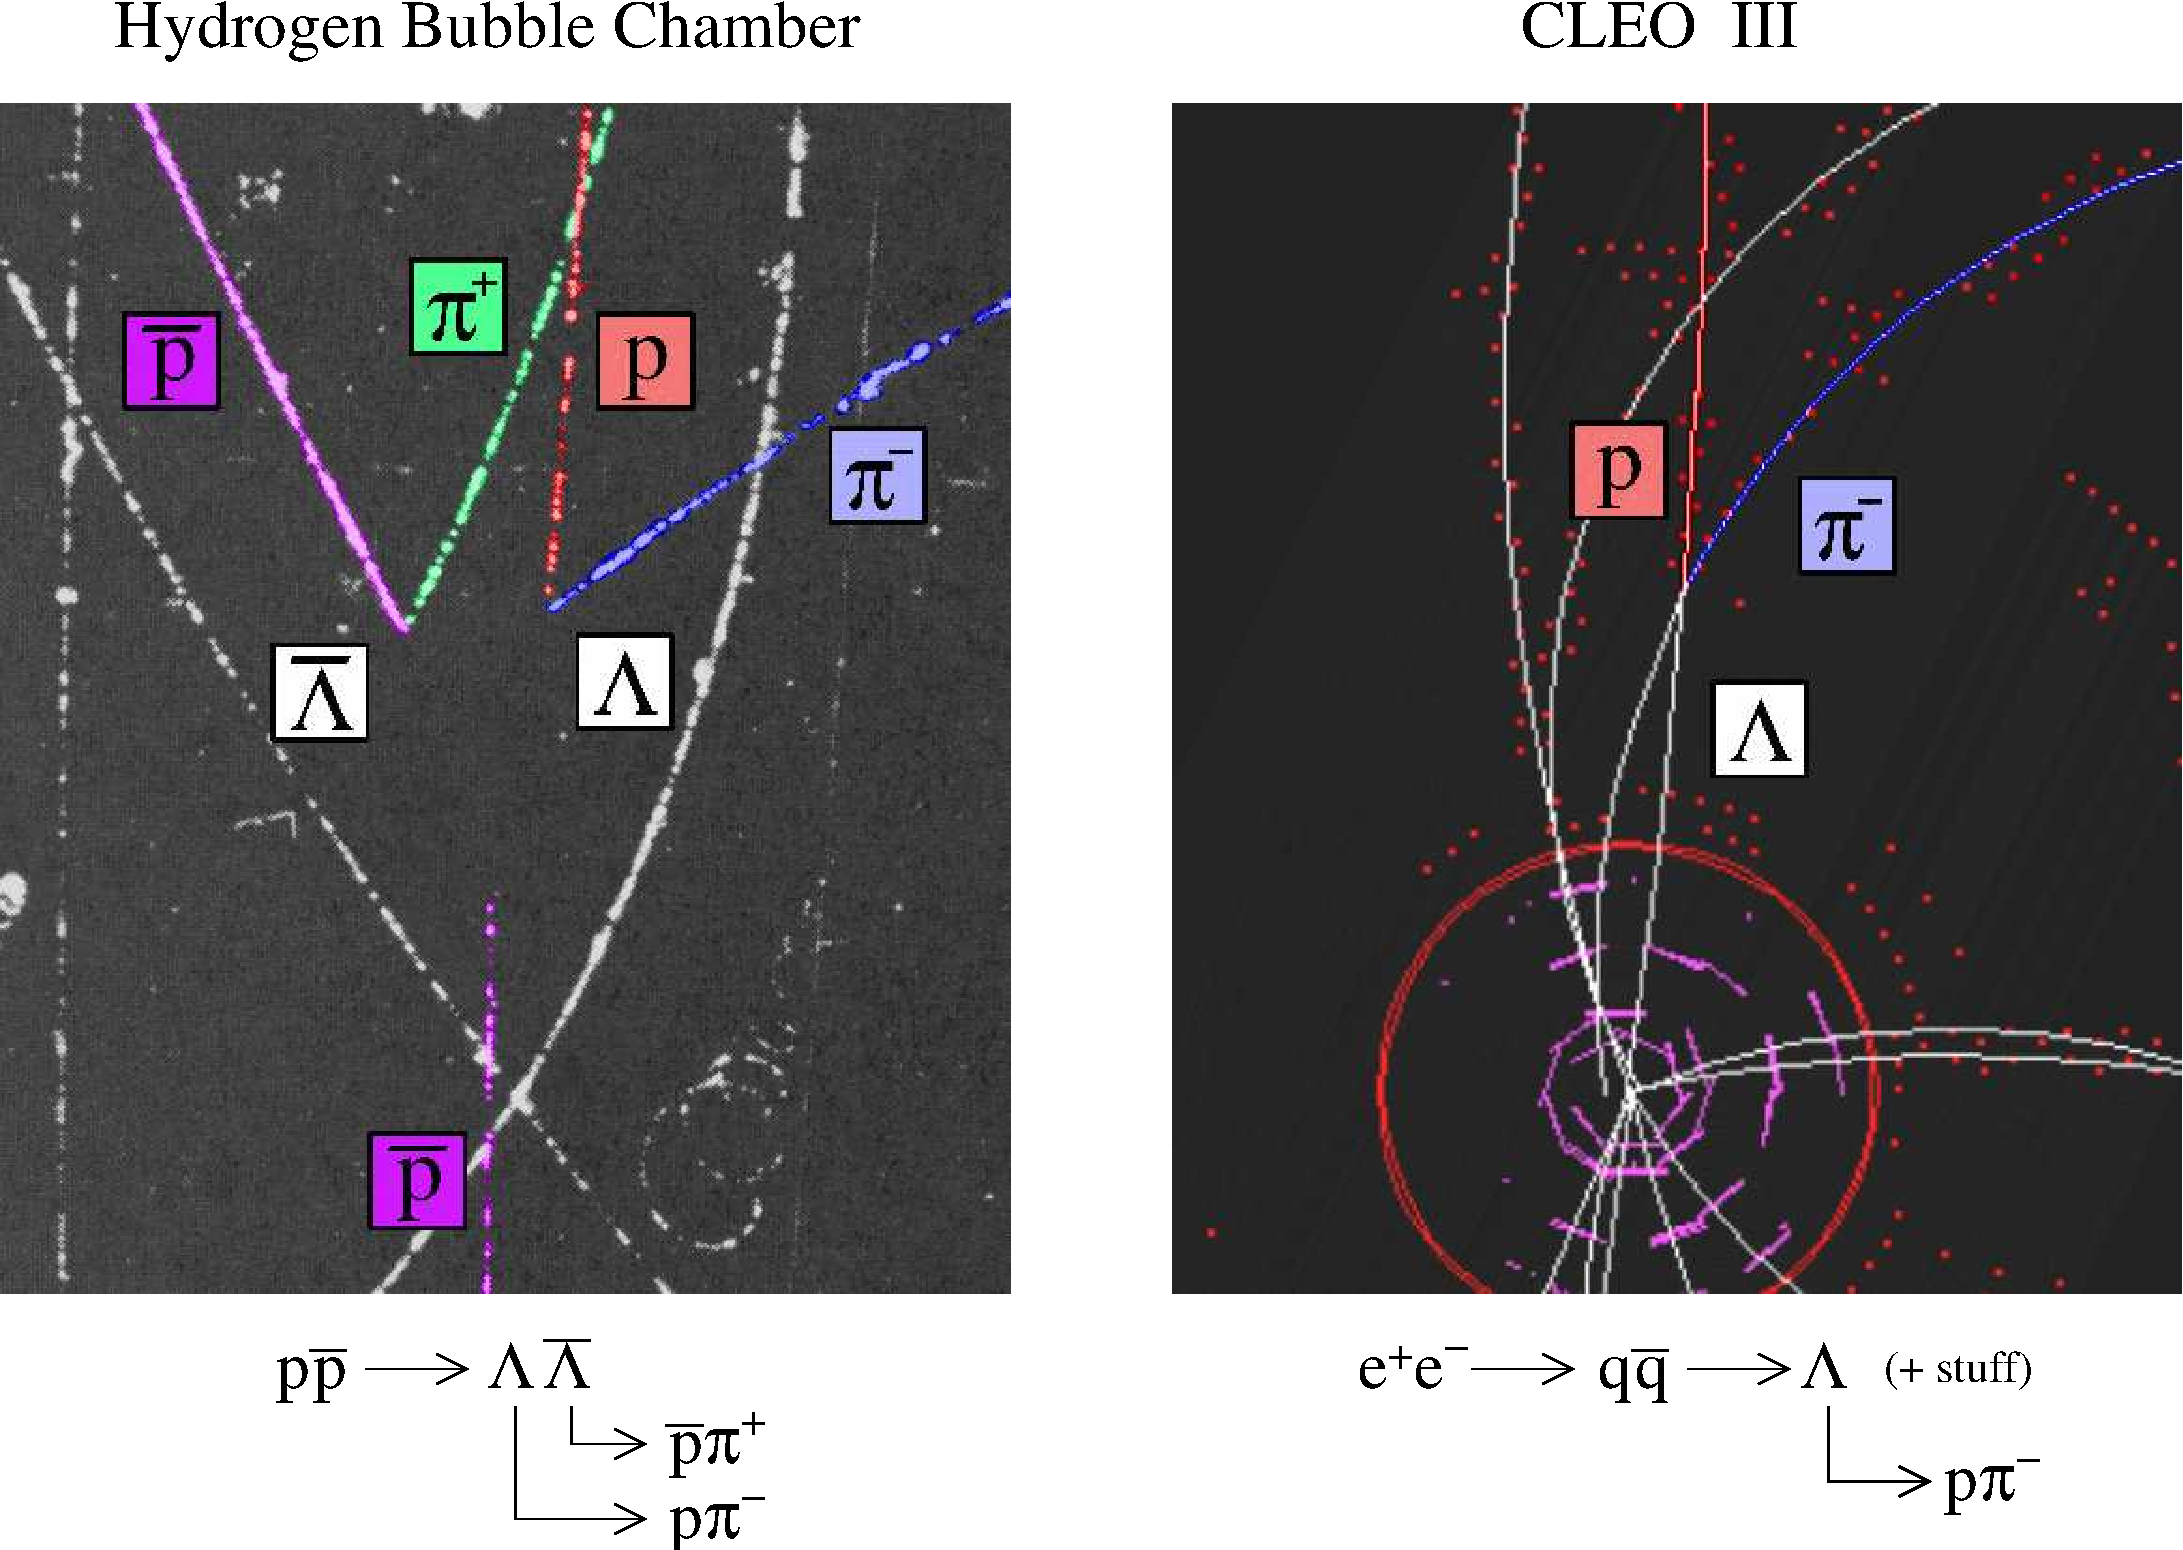
\includegraphics[width=0.55\linewidth]{2lambdas_sidebyside_small}
  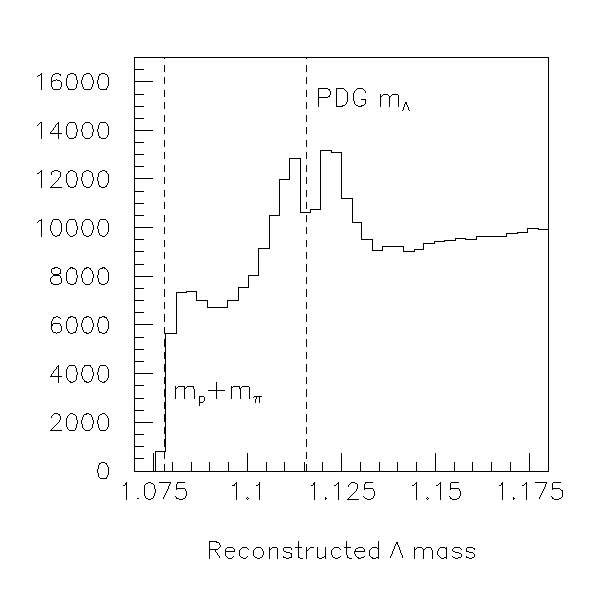
\includegraphics[width=0.4\linewidth]{lambdamass}
\end{center}

\begin{enumerate}
  \item Find track intersections far from the origin (hint: simplify
    the tracks as straight lines in XY or something)
  \item Reconstruct $\Lambda$ mass from the two observed tracks (for
    $K^0_S$, replace $m_p$ with $m_\pi$)
\[ {m_\Lambda}^2 = {E_\Lambda}^2 - \mbox{$\vec{p}_\Lambda$}^2 = \left(\sqrt{\left|{\vec{p}_p}\right|^2 + {m_p}^2} + \sqrt{\left|{\vec{p}_\pi}\right|^2 + {m_\pi}^2}\right)^2 - \left| \, \vec{p}_p + \vec{p}_\pi \, \right|^2 \\ \]
  \item What did I do wrong in my plot?  Why the double-peak?
\end{enumerate}
\end{slide}

\end{document}
